\documentclass{beamer}

% basic
\usepackage{comment}
\makeatletter
\@ifclassloaded{revtex4-2}{}{
	\@ifclassloaded{standalone}{}{
		\@ifclassloaded{beamer}{}{
			\usepackage{geometry} % only use geometry outside of RevTeX and TeXit
		}
	}
}
\@ifclassloaded{beamer}{}{
	\usepackage{titlesec}
}
\makeatother
\usepackage{microtype}
\usepackage[dvipsnames]{xcolor}
\usepackage{titlesec}

% programmability
\usepackage{xparse}
\usepackage{xtemplate}
\usepackage{ifthen}
\usepackage{xintexpr}
\usepackage{mathcommand}

% Support for CJK characters
\ifthenelse{\equal{\meaning\pdftexbanner}{\meaning\someundefinednonsense}}{
	\ifthenelse{\equal{\meaning\luatexbanner}{\meaning\someundefinednonsense}}{
		% xelatex
		\usepackage{xeCJK}
	}{
		% lualatex
	}
}{
	% pdflatex
	\usepackage{CJKutf8}
	\AddToHook{begindocument/end}{\CJK{UTF8}{gbsn}}
	\AddToHook{enddocument}{\endCJK}
}

% fonts
\usepackage{amsfonts} % for \mathbb, \mathfrak
\usepackage{mathrsfs} % for \mathscr
\usepackage{bm}
\usepackage{upgreek}

\newcommand{\mbb}[1]{\mathbb{#1}}
\newcommand{\mfk}[1]{\mathfrak{#1}}
\newcommand{\mrm}[1]{\mathrm{#1}}
\newcommand{\trm}[1]{\textrm{#1}}
\newcommand{\mbf}[1]{\mathbf{#1}}
\newcommand{\tbf}[1]{\textbf{#1}}
%\newcommand{\mit}[1]{\mathit{#1}}
\newcommand{\msf}[1]{\mathsf{#1}}
\newcommand{\mcal}[1]{\mathcal{#1}}
\newcommand{\mscr}[1]{\mathscr{#1}}
%\newcommand{\mtt}[1]{\mathtt{#1}}
\newcommand{\tit}[1]{\textit{#1}}
\newcommand{\ttt}[1]{\texttt{#1}}
\newcommand{\bs}[1]{\boldsymbol{#1}}

% basic utilities
\usepackage{mathtools}
\usepackage{amsthm}
\usepackage{verbatim}
\usepackage{lipsum}

% extensions
\usepackage{cancel} % \cancel
\usepackage{tensor} % \tensor, \indices
\usepackage{fixdif} % \d
\usepackage[shortlabels,inline]{enumitem} % options to enumerate and itemize environments
\usepackage{dcolumn} % align numbers by decimal point in tabular
\usepackage{hyperref} % \url, \href, and add hyperlinks to crossrefs
\usepackage{scalerel} % \scalerel, \stretchrel, \scaleto, \stretchto
\usepackage[notquote]{hanging} % \hangpara
\usepackage{chngcntr} % \counterwithin, \counterwithout
\usepackage{slashed} % \slashed
\usepackage{csquotes} % displayquote environment
\usepackage{xspace} % \xspace

\makeatletter
\@ifclassloaded{beamer}{
	% https://tex.stackexchange.com/a/24491
	\setitemize{label=\usebeamerfont*{itemize item}%
	\usebeamercolor[fg]{itemize item}
	\usebeamertemplate{itemize item}}
}{}
\makeatother

% beamer style
\makeatletter
\@ifclassloaded{beamer}{
	\usetheme{Boadilla}
	\usefonttheme{serif}
	\setbeamertemplate{footline}{% https://tex.stackexchange.com/a/67000
		\leavevmode%
		\hbox{%
			\begin{beamercolorbox}[wd=.2\paperwidth,ht=2.25ex,dp=1ex,center]{author in head/foot}%
				\usebeamerfont{author in head/foot}\insertshortauthor
			\end{beamercolorbox}%
			\begin{beamercolorbox}[wd=.8\paperwidth,ht=2.25ex,dp=1ex,center]{title in head/foot}%
				\usebeamerfont{title in head/foot}\insertshorttitle\hspace*{3em}
				\insertframenumber{} / \inserttotalframenumber\hspace*{1ex}
			\end{beamercolorbox}
		}%
		\vskip0pt%
	}
}{}

% floats
\usepackage{listings}
\lstdefinestyle{mystyle}{
	basicstyle=\ttfamily\scriptsize,
	tabsize=2,
	showspaces=false,
	showstringspaces=false,
	extendedchars=true,
	breaklines=true,
	postbreak=\mbox{$\hookrightarrow$\space}
}
\lstset{style=mystyle}

\makeatletter
\@ifclassloaded{revtex4-2}{
	% https://tex.stackexchange.com/a/597712
	\usepackage[caption=false]{subfig}
	\usepackage{ragged2e}
	\DeclareCaptionJustification{justified}{\justifying}
}{
	\usepackage{caption} % not compatible with RevTeX
	\usepackage{subfig}
}
\makeatother

\usepackage{graphicx} % \includegraphics
\usepackage{booktabs} % \toprule, \midrule, \bottomrule
\setlength{\tabcolsep}{12pt}

% fancy tools
\usepackage[version=4]{mhchem}
\usepackage{chemfig}
\usepackage{chemmacros}

\usepackage{physics2}
\usephysicsmodule[empty={}]{diagmat}
\usephysicsmodule{doubleprod}
\usephysicsmodule{xmat}

\usepackage[separate-uncertainty=true,multi-part-units=single]{siunitx}
\sisetup{range-phrase=--, range-units=single} % use -- for ranges, unit appears only once
\catcode`\%=12\relax
\DeclareSIUnit[number-unit-product=]\percent{%}
\catcode`\%=14\relax % use \percent in \SI{}{}
\DeclareSIUnit[number-unit-product=\,]\fahrenheit{\SIUnitSymbolDegree F} % \fahrenheit

% symbols
\usepackage{amssymb}
\usepackage[nointegrals]{wasysym}
\usepackage[safe]{tipa}

\usepackage{pifont}
\newcommand{\cmark}{\text{\ding{51}}}
\newcommand{\xmark}{\text{\ding{55}}}

\newcommand{\bN}{\mbb{N}}
\newcommand{\bC}{\mbb{C}}
\newcommand{\bR}{\mbb{R}}
\newcommand{\bQ}{\mbb{Q}}
\newcommand{\bZ}{\mbb{Z}}

\newcommand{\alp}{\alpha}
\newcommand{\gma}{\gamma}
\newcommand{\Gma}{\Gamma}
\newcommand{\dlt}{\delta}
\newcommand{\Dlt}{\Delta}
\newcommand{\eps}{\epsilon}
\newcommand{\veps}{\varepsilon}
\newcommand{\vphi}{\varphi}
\newcommand{\tht}{\theta}
\newcommand{\Tht}{\Theta}
\newcommand{\kap}{\kappa}
\newcommand{\lmd}{\lambda}
\newcommand{\Lmd}{\Lambda}
\newcommand{\sgm}{\sigma}
\newcommand{\Sgm}{\Sigma}
\newcommand{\omg}{\omega}
\newcommand{\Omg}{\Omega}

\newcommand{\divby}{\divisionsymbol}
\newcommand{\ceq}{\coloneqq}
\newcommand{\eqc}{\eqqcolon}

\renewmathcommand{\i}{\mrm{i}}
\newcommand{\e}{\mrm{e}}
\newcommand{\st}{\trm{s.t.}}

\NewChemParticle{\muon}{\chemmu}
\NewChemParticle{\tauon}{\chemtau}
\NewChemParticle{\eneu}{\chemnu_{\!\!e}}
\NewChemParticle{\mneu}{\chemnu_{\!\!\chemmu}}
\NewChemParticle{\tneu}{\chemnu_{\!\!\chemtau}}
\NewChemParticle{\pion}{\chempi}
\NewChemParticle{\etaon}{\chemeta}

% for drawing
\usepackage{tikz-cd}
\usepackage{circuitikz}
\usepackage{pgfplots}
\usepackage{tikz-3dplot}
%\usepackage{tikz-feynhand}

\usetikzlibrary{intersections}
\usetikzlibrary{decorations.markings}
\usetikzlibrary{decorations.pathmorphing}
\usetikzlibrary{arrows.meta}
\usetikzlibrary{calc}
\usetikzlibrary{bending}
\usetikzlibrary{patterns}
\usetikzlibrary{positioning}
\usetikzlibrary{math}
\usetikzlibrary{pgfplots.units}
\usetikzlibrary{angles}
\usetikzlibrary{shapes.geometric}
\usetikzlibrary{shadings}

\pgfplotsset{
	compat=newest,
	ylabel style={rotate=-90},
	trig format=rad
}
% https://tex.stackexchange.com/a/685953
\makeatletter
\patchcmd\pgfpatharc{\pgfutil@in@}{%
	\pgfmathiftrigonometricusesdeg{}{%
		\pgfmathradians@{\pgf@temp@a}\let\pgf@temp@a\pgfmathresult
		\pgfmathradians@{\pgf@temp@b}\let\pgf@temp@b\pgfmathresult
		\def\pgfmath@trig@format@choice{0}
	}\pgfutil@in@}{}{\PatchFailed}
\makeatother

% more shortcuts
\newcommand{\mcl}{\mathclap}
\newcommand{\mll}{\mathllap}
\newcommand{\mrl}{\mathrlap}
\newcommand{\fr}{\frac}
\newcommand{\dfr}{\dfrac}
\newcommand{\tfr}{\tfrac}
\newcommand{\opn}{\operatorname}
\newcommand{\bhat}[1]{\hat{\bs{\mbf{#1}}}}
\newcommand{\fs}{\slashed}
\newcommand{\hatfs}[1]{{\hat{\phantom{#1}}\mathllap{\fs{#1}}}}
\newcommand{\func}[3]{#1\colon#2\to#3} % \func{f}{A}{B} => f:A->B
\newcommand{\vfunc}[5]{\func{#1}{#2}{#3},\quad#4\longmapsto#5} % \vfunc{f}{A}{B}{a}{b} => f:A->B, a|->b
\newcommand{\fc}[2]{#1\mathchoice{\!}{\!}{}{}\p{#2}} % \fc{f}{x} => f(x)
\newcommand{\bfc}[2]{#1\mathchoice{\!}{\!}{}{}\b{#2}} % \bfc{f}{x} => f[x]
\newcommand{\Bfc}[2]{#1\mathchoice{\!}{\!}{}{}\B{#2}} % \bfc{f}{x} => f{x}
\newcommand{\opc}[2]{\fc{\opn{#1}}{#2}} % \opc{sgn}{x} => sgn(x)
\newcommand{\bopc}[2]{\bfc{\opn{#1}}{#2}} % \bopc{sgn}{x} => sgn[x]
\newcommand{\Bopc}[2]{\Bfc{\opn{#1}}{#2}} % \bopc{sgn}{x} => sgn{x}
\newcommand{\set}[2]{\left\{#1\;\middle|\;#2\right\}} % \set{x}{S} => {x|S}
\newcommand{\tp}[3][]{
	\ifthenelse{\equal{#1}{}}
	{\fr{\partial#2}{\partial#3}}{\p{\fr{\partial#2}{\partial#3}}_{#1}}
} % \tp[a]{f}{x} => (df/dx)_a, \tp{f}{x} => df/dx
\newcommand{\abar}[2]{\left.#1\right|_{#2}} % \abar{f}{a} => f|_a
\newcommand{\order}[1]{\fc{\mrm{O}}{#1}} % \order{x} => O(x)

% parentheses
\renewmathcommand\p[1]{\left(#1\right)}
\newcommand\B[1]{\left\{#1\right\}}
\newcommand\V[1]{\left\lVert#1\right\rVert}
\renewmathcommand\b[1]{\left[#1\right]}
\renewmathcommand\v[1]{\left|#1\right|}
\renewmathcommand\a[1]{\left\langle#1\right\rangle}
\newcommand\floor[1]{\left\lfloor#1\right\rfloor}
\newcommand\ceil[1]{\left\lceil#1\right\rceil}
\newcommand\round[1]{\left\lfloor#1\right\rceil}
\newcommand\bra[1]{\left<#1\right|}
\newcommand\ket[1]{\left|#1\right>}
\newcommand\braket[2]{\left<#1\middle|#2\right>}
\newcommand\mel[3]{\left<#1\middle|#2\middle|#3\right>}
\newcommand\bbra[1]{\left[#1\right|}
\newcommand\bket[1]{\left|#1\right]}
\newcommand\bbraket[2]{\left[#1\middle|#2\right]}
\newcommand\bmel[3]{\left[#1\middle|#2\middle|#3\right]}
\newcommand\bmela[3]{\left[#1\middle|#2\middle|#3\right>}
\newcommand\amelb[3]{\left<#1\middle|#2\middle|#3\right]}

% operators
\DeclareMathOperator{\sech}{sech}
\DeclareMathOperator{\csch}{csch}
\DeclareMathOperator{\arsinh}{arsinh}
\DeclareMathOperator{\arcosh}{arcosh}
\DeclareMathOperator{\artanh}{artanh}
\DeclareMathOperator{\arcoth}{arcoth}
\DeclareMathOperator{\arsech}{arsech}
\DeclareMathOperator{\arcsch}{arcsch}
\DeclareMathOperator{\sgn}{sgn}
\DeclareMathOperator{\nint}{nint}
\DeclareMathOperator{\PV}{PV}
\let\Re\relax
\let\Im\relax
\DeclareMathOperator{\Re}{Re}
\DeclareMathOperator{\Im}{Im}
\DeclareMathOperator{\Tr}{Tr}
\DeclareMathOperator*{\bigTr}{Tr}
\DeclareMathOperator*{\bigdet}{det}
\DeclareMathOperator*{\argmax}{arg\,max}
\DeclareMathOperator*{\argmin}{arg\,min}
\DeclareMathOperator*{\Res}{Res}
\DeclareMathOperator*{\supp}{supp}
\letdif\dt{delta}
\letdif\Dt{Delta}

% Lie groups and others
\renewmathcommand\O[1]{\fc{\mrm O}{#1}}
\newcommand\SO[1]{\fc{\mrm{SO}}{#1}}
\newcommand\U[1]{\fc{\mrm U}{#1}}
\newcommand\SU[1]{\fc{\mrm{SU}}{#1}}
\newcommand\GL[1]{\fc{\mrm{GL}}{#1}}
\newcommand\SL[1]{\fc{\mrm{SL}}{#1}}
\newcommand\Spin[1]{\fc{\mrm{Spin}}{#1}}
\newcommand\Pin[1]{\fc{\mrm{Pin}}{#1}}
\newcommand\Cl[1]{\fc{\mrm{Cl}}{#1}}

\renewmathcommand\o[1]{\fc{\mfk o}{#1}}
\newcommand\so[1]{\fc{\mfk{so}}{#1}}
\newcommand\su[1]{\fc{\mfk{su}}{#1}}
\newcommand\gl[1]{\fc{\mfk{gl}}{#1}}
\renewmathcommand\sl[1]{\fc{\mfk{sl}}{#1}}
\newcommand\spin[1]{\fc{\mfk{spin}}{#1}}
\newcommand\pin[1]{\fc{\mfk{pin}}{#1}}

% theorems
\makeatletter
\@ifclassloaded{beamer}{}{
	\newtheorem{theorem}{Theorem}
	\newtheorem{proposition}{Theorem}
	\newtheorem{lemma}[theorem]{Lemma}
	\newtheorem{corollary}[theorem]{Corollary}\theoremstyle{definition}
	\newtheorem{definition}[theorem]{Definition}
}
\makeatother

% displaystyle matrices
\makeatletter
\def\env@dmatrix{
	\hskip-\arraycolsep
	\let\@ifnextchar\new@ifnextchar
	\extrarowheight=2ex
	\array{*\c@MaxMatrixCols{>{\displaystyle}c}}
}
\newenvironment{dmatrix}{\env@dmatrix}{\endarray\hskip-\arraycolsep}
\newenvironment{pdmatrix}{\left(\env@dmatrix}{\endmatrix\right)}
\newenvironment{bdmatrix}{\left[\env@dmatrix}{\endmatrix\right]}
\newenvironment{Bdmatrix}{\left\{\env@dmatrix}{\endmatrix\right\}}
\newenvironment{vdmatrix}{\left|\env@dmatrix}{\endmatrix\right|}
\newenvironment{Vdmatrix}{\left\lVert\env@dmatrix}{\endmatrix\right\rVert}
\makeatother

\title{The broken stick problem as the continuum limit of a Bernoulli process}
\author{Ulysses Zhan\inst{1}}
\institute{\inst{1} Department of Physics, University of California, Santa Barbara}
\date{May 13, 2026}

\begin{document}

\begin{frame}
	\titlepage
\end{frame}

\begin{frame}{Run}
	A \tbf{run} is consecutive identical elements in a sequence.

	Sequence of Bernoulli trials:
	\[\newmoon\;\newmoon\;\fullmoon\;\fullmoon\;\fullmoon\;\newmoon\;\fullmoon\;\newmoon\;\newmoon\;\newmoon\;\fullmoon\;\fullmoon
	\;\newmoon\;\newmoon\;\fullmoon\;\fullmoon\;\fullmoon\;\fullmoon\;\newmoon\;\newmoon\;\newmoon\;\newmoon\;\newmoon\]
	Run of ``$\newmoon$'':
	\[\boxed{\newmoon\;\newmoon}\fullmoon\;\fullmoon\;\fullmoon\boxed\newmoon\fullmoon\boxed{\newmoon\;\newmoon\;\newmoon}\fullmoon\;\fullmoon
	\boxed{\newmoon\;\newmoon}\fullmoon\;\fullmoon\;\fullmoon\;\fullmoon\boxed{\newmoon\;\newmoon\;\newmoon\;\newmoon\;\newmoon}\]
	The length of the longest run is $5$.
\end{frame}

\begin{frame}{The Research Question}
	Behavior of the longest run when sequence length $n\to\infty$
	while the probability of getting a perfect sequence is constant:
	\[n\to\infty,\]
	\[p^n=P=\mrm{const}.\]
\end{frame}

\begin{frame}{The Discrete Model}
	Consider a Bernoulli sequence of length $n$,
	where each element is either success (S) or failure (F),
	with probabilities $p$ and $1-p$ respectively, and independent of each other.
	Let $\fc{P_{n,k}}{p}$ be the probability that the length of the longest run of S's is $k$.
	What is the expression of $\fc{P_{n,k}}{p}$?
\end{frame}

\begin{frame}{The Recurrence Relation}
	\[\underbrace{\newmoon\,\newmoon\,\cdots\,\newmoon}_{k,k}
	\fullmoon
	\underbrace{\fullmoon\,\newmoon\,\cdots\,\fullmoon\,\newmoon}_{n-k-1,s<k}
	\qquad p^k\p{1-p}\sum_{s=0}^{k}P_{n-k-1,s}\]
	\[\underbrace{\newmoon\,\newmoon\,\cdots\,\newmoon}_{s,s<k}
	\fullmoon
	\underbrace{\fullmoon\,\newmoon\,\cdots\,\fullmoon\,\newmoon}_{n-s-1,k}
	\qquad \sum_{s=0}^{k-1}p^s\p{1-p}P_{n-s-1,k}\]
	\vfill
	\[P_{n,0<k<n}
	=\p{1-p}\p{p^k\sum_{s=0}^kP_{n-k-1,s}
	+\sum_{s=0}^{k-1}p^sP_{n-s-1,k}}.\]
	\[P_{n,0}=\p{1-p}^n,\qquad P_{n,n}=p^n,\qquad P_{n,k>n}=0.\]
\end{frame}

\begin{frame}{Visualizing the Discrete Distribution}
	\centering
	\includegraphics{../plot/n50.pdf}
\end{frame}

\begin{frame}{Defining the Continuum Limit}
	Define $P\ceq p^n$ and keep it constant as $n\to\infty$.
	The probability distribution of $x\ceq k/n$ is
	\[\fc f{P,x}\ceq\lim_{n\to\infty}n\fc{P_{n,xn}}{P^{1/n}}\qquad\p{0\le P\le1,\quad x\ge0}.\]
\end{frame}

\begin{frame}{The Integral Equation}
	\[\fc g{P,x}\ceq\fr1P\fc f{P,x}-\fc\dlt{x-1}.\]
	\vfill
	\[\begin{split}
		\fc g{P,0\le x\le1}&=-\ln P\left(
		\int_0^{x/\p{1-x}}\p{\fc g{P^{1-x},u}+\fc\dlt{u-1}}\d u
		\right.\\
		&\phantom{{}=}\left.{}+\int_x^{x/\p{1-x}}\p{\fc g{P^{x/v},v}+\fc\dlt{v-1}}\fr{\d v}v\right),\\
		\fc g{P,x>1}&=0.
	\end{split}\]
	\[\int_0^\infty\fc g{P,x}\d x=\fr1P-1.\]
\end{frame}

\begin{frame}{Overview of the ADM}
	The Adomian decomposition method (ADM):
	\[g=\fc\Phi g.\]
	\vfill
	\[g=g_0+\lmd g_1+\lmd^2 g_2+\lmd^3 g_3+\cdots,\]
	\[\fc\Phi g=\Phi_0+\lmd\fc{\Phi_1}g+\lmd^2\fc{\Phi_2}{g,g}
	+\lmd^3\fc{\Phi_3}{g,g,g}+\cdots.\]
	\vfill
	\[g_j=\sum_{l=0}^j\sum_{m_1+\cdots+m_l=j-l}\fc{\Phi_l}{g_{m_1},\ldots,g_{m_l}}.\]
\end{frame}

\begin{frame}{Piece-by-Piece Solution}
	\[\fc{g^{\p q}}{P,x}\ceq\fc g{P,x}\qquad\p{\fr1{q+1}<x<\fr1q}.\]
	\vfill
	\centering
	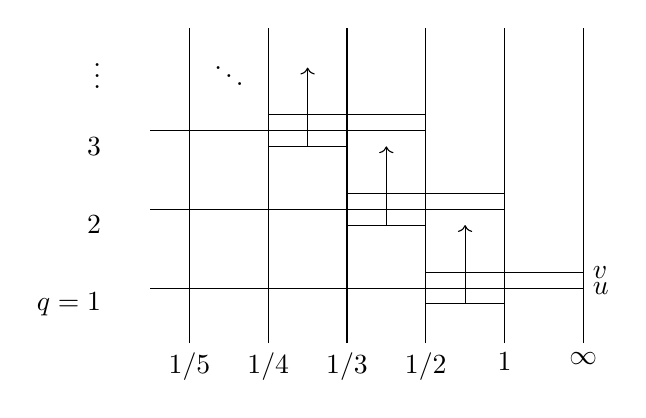
\begin{tikzpicture}
		\draw (-5,0.5) node[below] {$1/5$} -- (-5,4.5);
		\draw (-4,0.5) node[below] {$1/4$} -- (-4,4.5);
		\draw (-3,0.5) node[below] {$1/3$} -- (-3,4.5);
		\draw (-2,0.5) node[below] {$1/2$} -- (-2,4.5);
		\draw (-1,0.5) node[below] {$1$} -- (-1,4.5);
		\draw (-0,0.5) node[below] {$\infty$} -- (-0,4.5);
		\node[left] at (-6,1) {$q=1$};
		\draw (-1,1) -- (-2,1);
		\draw[->] (-1.5,1) -- (-1.5,2);
		\draw (0,1.2) node[right] {$u$} -- (-5.5,1.2);
		\draw (0,1.4) node[right] {$v$} -- (-2,1.4);
		\node[left] at (-6,2) {$2$};
		\draw (-2,2) -- (-3,2);
		\draw[->] (-2.5,2) -- (-2.5,3);
		\draw (-1,2.2) -- (-5.5,2.2);
		\draw (-1,2.4) -- (-3,2.4);
		\node[left] at (-6,3) {$3$};
		\draw (-3,3) -- (-4,3);
		\draw[->] (-3.5,3) -- (-3.5,4);
		\draw (-2,3.2) -- (-5.5,3.2);
		\draw (-2,3.4) -- (-4,3.4);
		\node[left] at (-6,4) {$\vdots$};
		\node at (-4.5,4) {$\ddots$};
	\end{tikzpicture}
\end{frame}

\begin{frame}{Solution}
	\[\fc F{P,x}\ceq\int_0^x\d x'\int_0^{x'}\d x''\,\fc f{P,x''},\quad r_s\ceq\ln P^{sx-1}.\]
	\[\fc F{P,x}=\fr P{\ln P}\sum_{s=1}^{\floor{1/x}}\fr{\p{-1}^s}{s!\,s}\e^{r_s}r_s^s
	-\fr{\opn{li}P-\gma-\fc\ln{-\ln P}}{\ln P}+x.\]
\end{frame}

\begin{frame}{Visualization of the Solution}
	\centering
	\includegraphics{../plot/compare.pdf}
\end{frame}

\begin{frame}{The Broken Stick Problem}
	Break a unit-length stick at $k$ random points. The distribution of the longest segment is
	$\fc{f_k}x$.
	\[\fc f{\e^{-\lmd},x}=\e^{-\lmd}\sum_{k=0}^\infty\fr{\lmd^k}{k!}\fc{f_k}x,\]
	\[\fc f{P,x}=P\sum_{k=0}^\infty\fr{\p{-\ln P}^k}{k!}\fc{f_k}x.\]
\end{frame}

\begin{frame}{Run Statistics to the Gumbel Distribution}
	$\fc f{P,x}$ tends to the Gumbel distribution as $P\to0$.
	\centering
	\includegraphics{../plot/Gumbel.pdf}
\end{frame}

\begin{frame}{Broken Stick Problem to the Gumbel Distribution}
	$\fc{f_k}x$ tends to the Gumbel distribution as $k\to\infty$.
	\centering
	\includegraphics{../plot/Gumbel_F_k.pdf}
\end{frame}

\begin{frame}{Summary of Findings}
	\begin{itemize}
		\item Derive a recurrence relation for the longest run distribution
		and formulate its continuum limit to an integral equation.
		\item Derive a piecewise analytical solution using the ADM.
		\item Formally establish the link between run statistics and the broken stick problem.
		\item Formally derive the Gumbel distribution in limiting cases.
	\end{itemize}
\end{frame}

\end{document}
